\documentclass[12pt]{article}

\usepackage{graphicx}

\title{CS 496 Lab 1: Wireshark}
\author{Ian Kronquist}

\begin{document}
\maketitle

\begin{enumerate}
    \item I was on a busy library wireless network so I saw all sorts of interesting packets. A few include TLSv1.2, HTTP, TCP, MDNS, ARP, and ICMP. \\
    \item The first HTTP GET packet was sent 6.015019 seconds after wireshark started, and the second was sent 6.042493 seconds after the program was started. It took a total of 0.027474 seconds to complete the request. \\
    \item My computer's IP address was 192.168.9.224. The UMass server's IP address was 128.119.245.12. \\
    \item Image of the packets captured:

\end{enumerate}

\begin{figure}[!ht]
    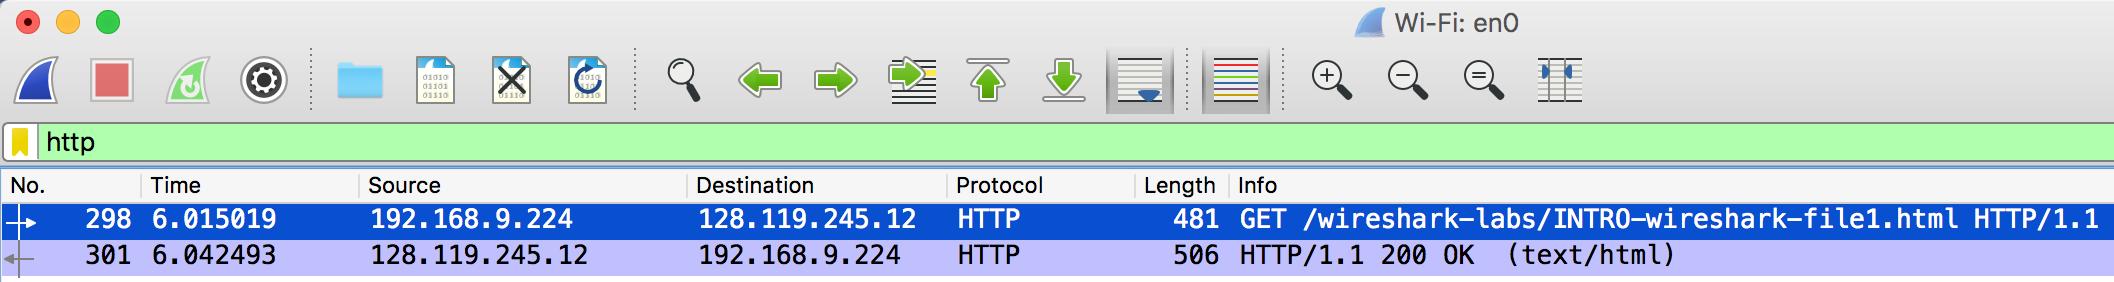
\includegraphics[scale=0.5]{./wireshark.png}
    \caption{Screenshot of wireshark packages captured}
\end{figure}


\end{document}
